\documentclass[12pt,a4paper,titlepage]{article}

\usepackage{preamble}

\title{Détection de la végétation à partir d'une image aérienne multi-spectrale}
\author{Saâd Aziz Alaoui, Yassine Jamoud, Samy Haffoudhi}
\date{\today}

\begin{document}

\maketitle

\section*{Introduction}

On dispose d'une image acquise dans trois bandes de fréquences choisies de sorte à pouvoir
identifier les surfaces au sol couvertes par de la végétation. L'objectif du TD est de
mettre en œuvre des algorithmes d'analyse de cette image multi-spectrale permettant de
détecter la végétation.

\section{Réponses aux questions}

\begin{enumerate}
    \item{Commençons par ouvrir l'image \texttt{camargue.jpg} dans Matlab.

        \begin{figure}[H]
            \caption{Image}
            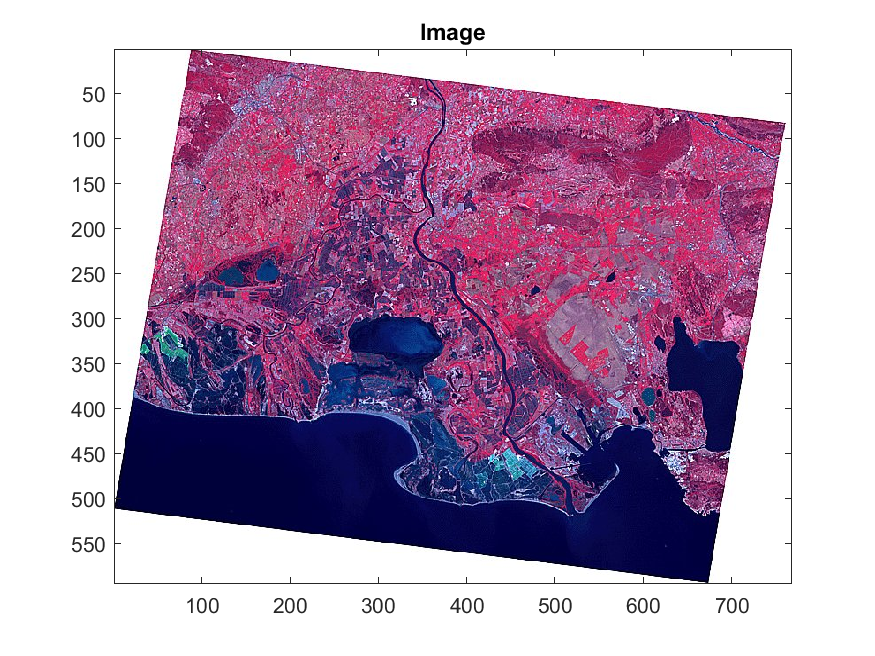
\includegraphics[width=.5\textwidth]{image}
            \centering
        \end{figure}

        Les couleurs de l'image affichée sont surprenantes. En effet on n'observe par exemple
        pas de vert alors qu'on cherche à identifier de la végétation. Ces couleurs
        s'expliquent par le fait que les valeurs des pixels ne correspondent pas à des
        intensités RVB.
        }

    \item{Affichons maintenant les trois canaux séparément :

        \begin{figure}[H]
            \caption{Les 3 canaux de l'image}
            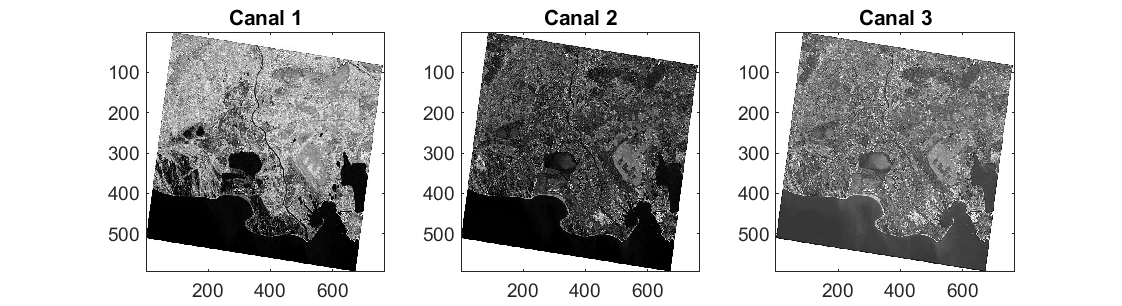
\includegraphics[width=\textwidth]{canaux}
            \centering
        \end{figure}

        En nous aidant du spectre de réflectance des végétaux on en déduit les correspondances
        suivantes :

        \begin{itemize}
            \item{Canal 1 $\longleftrightarrow$ Proche infrarouge}
            \item{Canal 2 $\longleftrightarrow$  Rouge}
            \item{Canal 3 $\longleftrightarrow$ Vert}
        \end{itemize}
        }

    \item{
            Affichons l'histogramme pour chaque canal :

            \begin{figure}[H]
                \caption{Canal 1}
                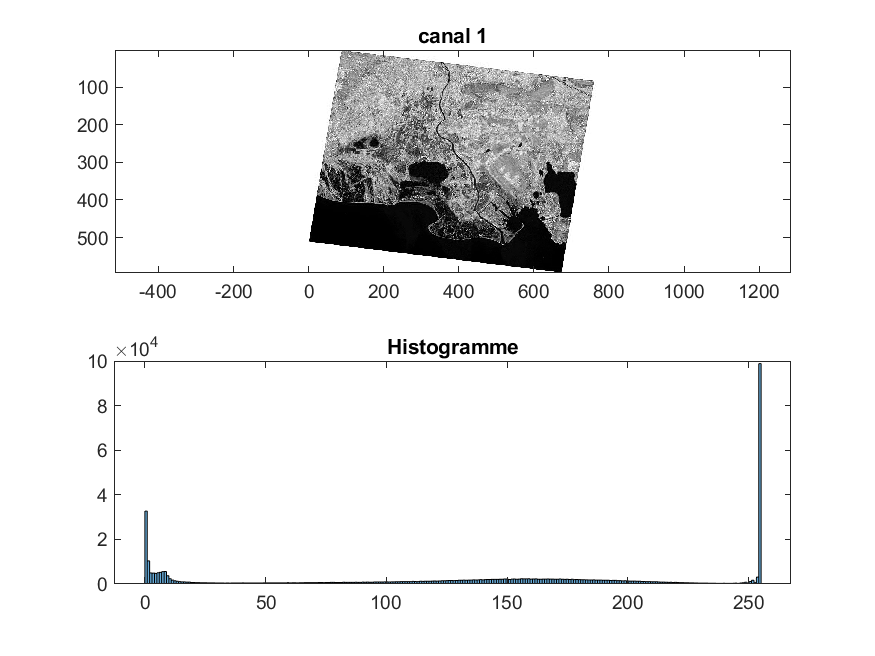
\includegraphics[width=.5\textwidth]{canal1}
                \centering
            \end{figure}

            \begin{figure}[H]
                \caption{Canal 2}
                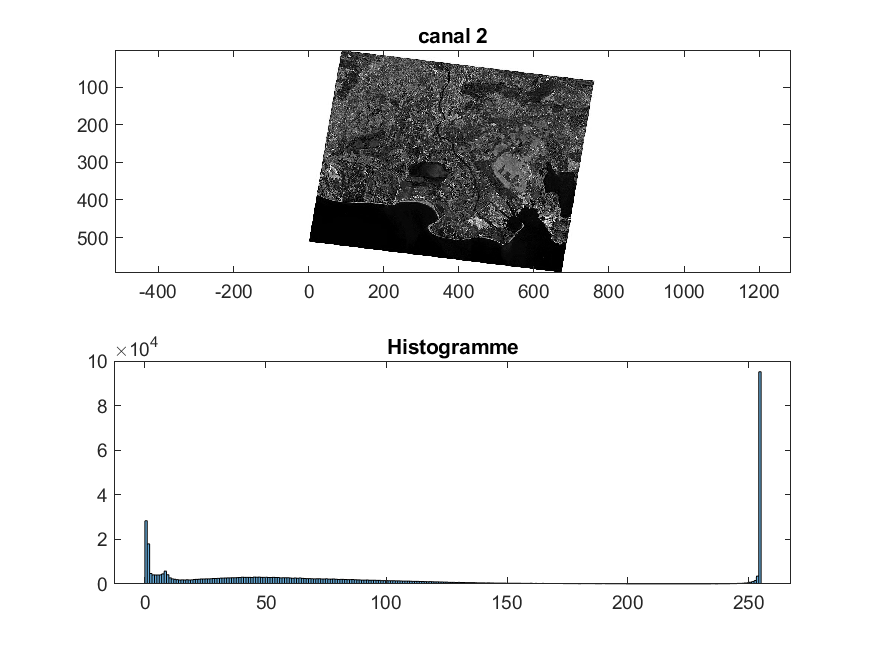
\includegraphics[width=.5\textwidth]{canal2}
                \centering
            \end{figure}

            \begin{figure}[H]
                \caption{Canal 3}
                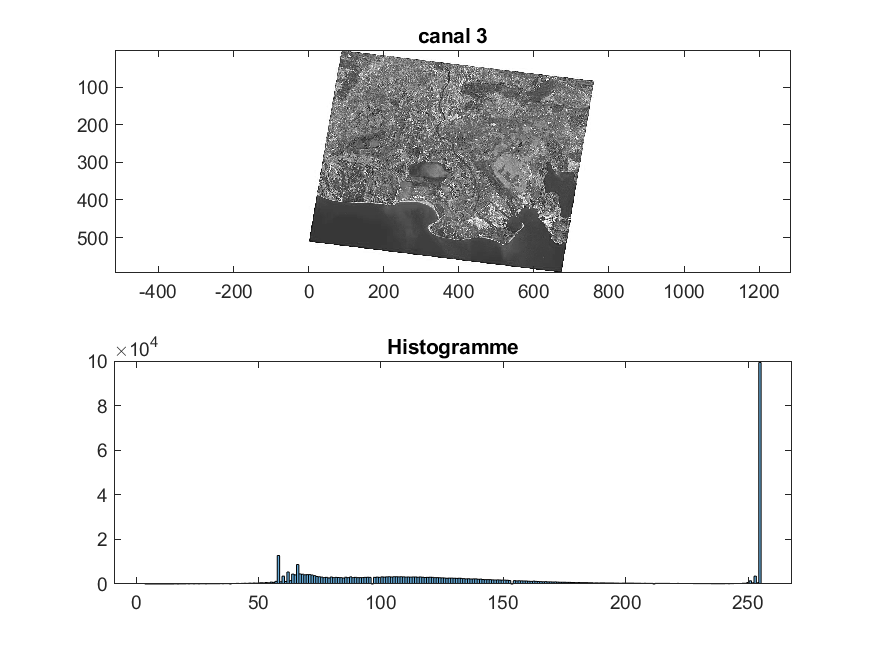
\includegraphics[width=.5\textwidth]{canal3}
                \centering
            \end{figure}

            On observe différents "clusters" dans les histogrammes, on peut essayer d'identifier
            la végétation par un seuillage. On choisit alors un seuil adapté pour chacun des
            trois canaux (On aurait aussi pu utiliser deux seuils par canal) de sorte à
            exclure les deux pics, on choisit par exemple respectivement les seuils, 2000, 1000
            et 1000.
        }

    \item{
            On appliquant le seuillage décrit plus haut, on obtient les masques suivants :

            \begin{figure}[H]
                \caption{Canal 1}
                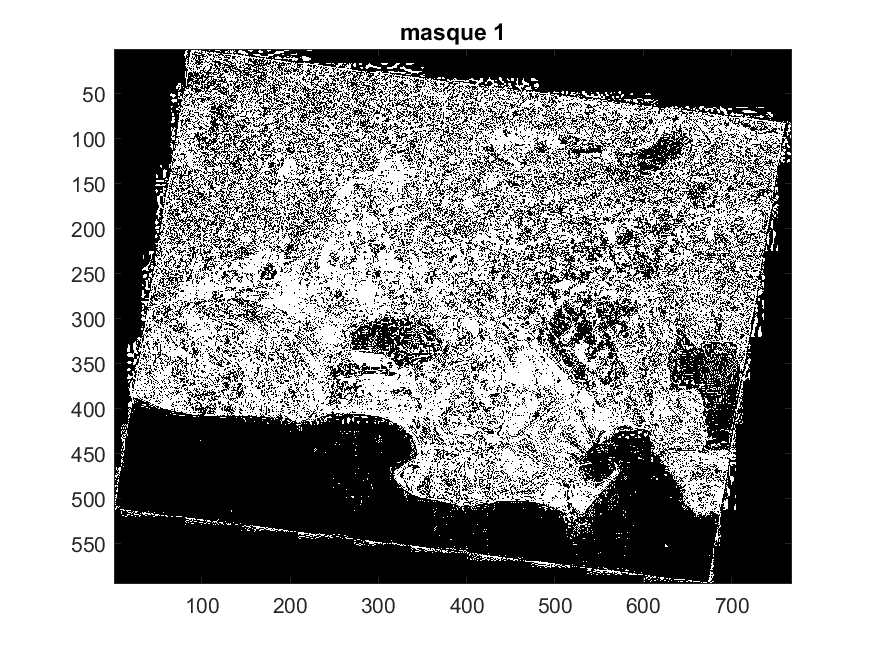
\includegraphics[width=.5\textwidth]{masque1}
                \centering
            \end{figure}

            \begin{figure}[H]
                \caption{Canal 2}
                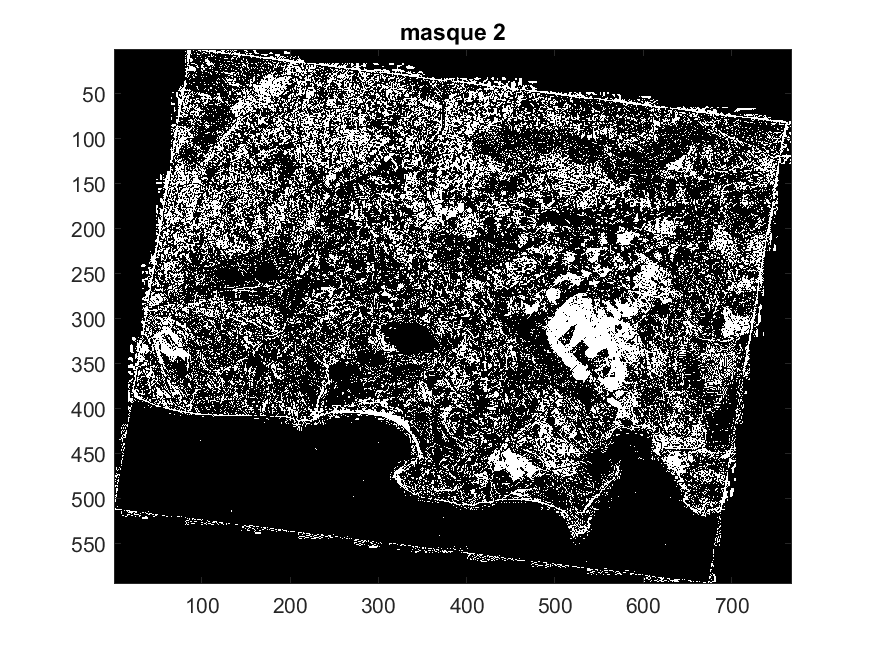
\includegraphics[width=.5\textwidth]{masque2}
                \centering
            \end{figure}

            \begin{figure}[H]
                \caption{Canal 3}
                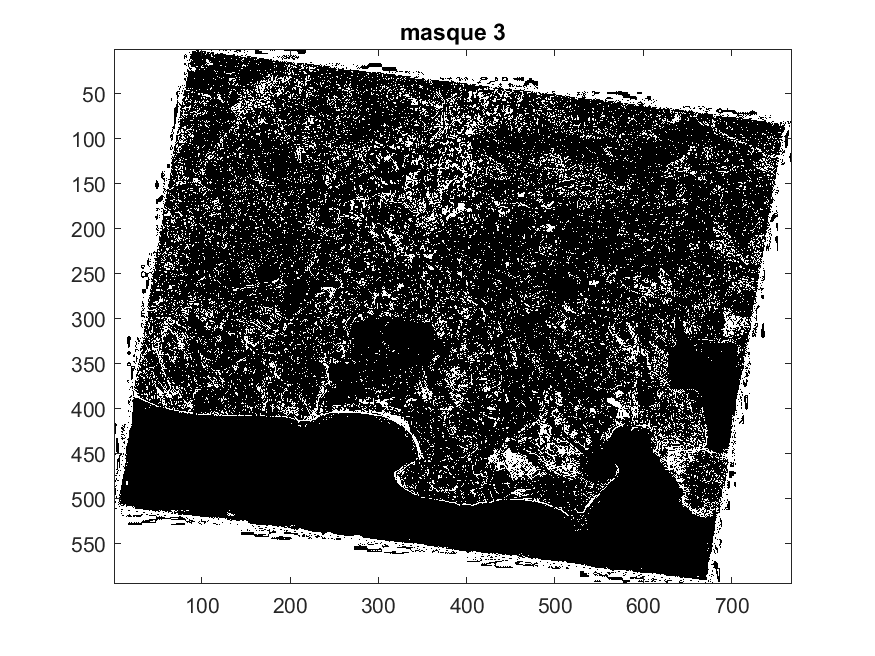
\includegraphics[width=.5\textwidth]{masque3}
                \centering
            \end{figure}

            On voit que pour cette première méthode les résultats varient beaucoup d'un
            canal à l'autre. Le masque 1 est celui sur lequel le plus de végétation serait
            identifiée tandis que le masque 3 est bien plus sélectif, le masque 2 est entre
            les deux. On en déduit qu'il faut mettre en place des méthodes plus robustes
            pour ce problème de détection.
        }

    \item{
            Rappel des bandes de longueurs d'onde :

            \begin{itemize}
                \item{Bleu : 300 à 500 nm}
                \item{Rouge : 600 à 800 nm}
                \item{Vert : 500 à 580 nm}
                \item{PIR : 0.8 à 2 $\mu$m}
            \end{itemize}

            Ainsi, d'après le graphique, la végétation se distingue le plus des autres
            éléments dans la bande PIR mais on peut encore le confondre avec le béton.
        }

    \item{
            Le NDVI est défini par : $$ NDVI = \frac{PIR - R}{PIR + R} $$
            Cet indice est adapté à la détection de la végétation car il prend en compte le
            domaine PIR où la végétation se distingue le plus et lui soustrait le canal R (avant
            de normaliser) où la végétation émet moins. Par exemple, le béton émet de
            manière quasiment identique entre ces deux domaines, on pourra alors le distinguer
            de la végétation à l'aide de l'indice. Par ailleurs, cet indice est aussi utilisé pour estimer
            l'état de santé de la végétation.
        }

    \item{
            Affichons l'image correspondante au DVI :

            \begin{figure}[H]
                \caption{DVI}
                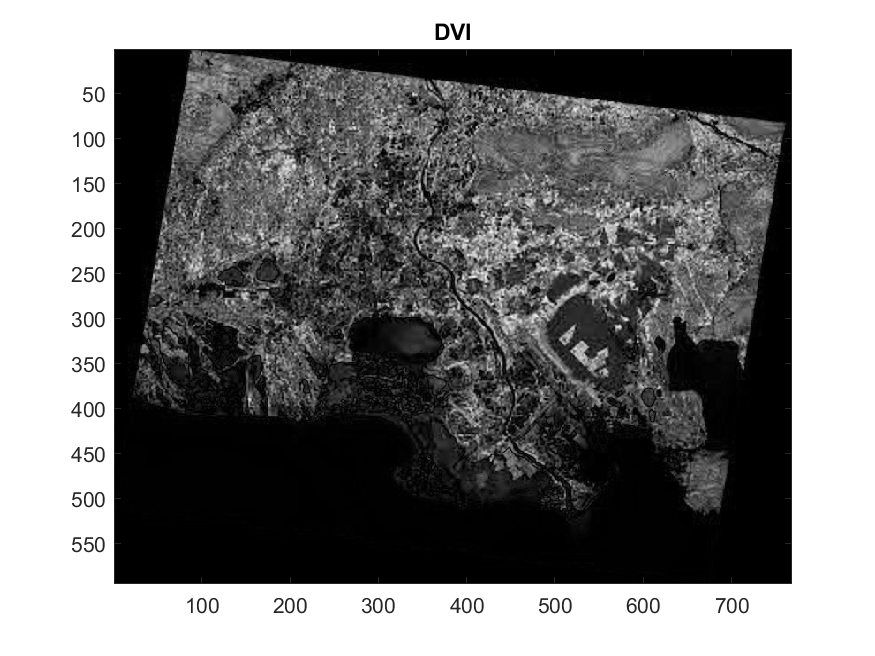
\includegraphics[width=.6\textwidth]{dvi}
                \centering
            \end{figure}

            Et l'histogramme correspondant :

            \begin{figure}[H]
                \caption{Histogramme}
                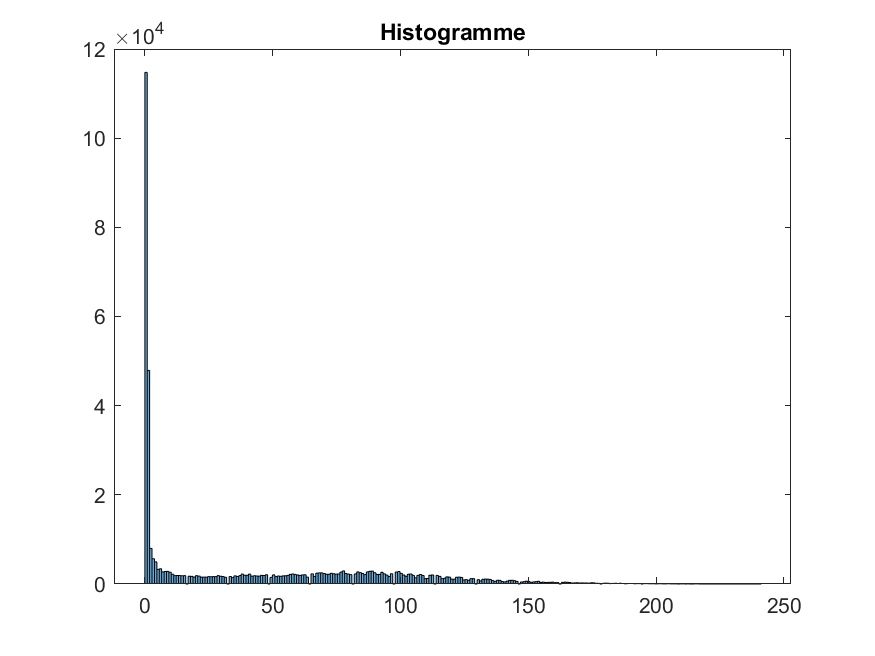
\includegraphics[width=.6\textwidth]{dvi_hist}
                \centering
            \end{figure}

            Enfin, représentons les masques obtenus pour différentes valeurs de seuil :

            \begin{figure}[H]
                \caption{Histogramme}
                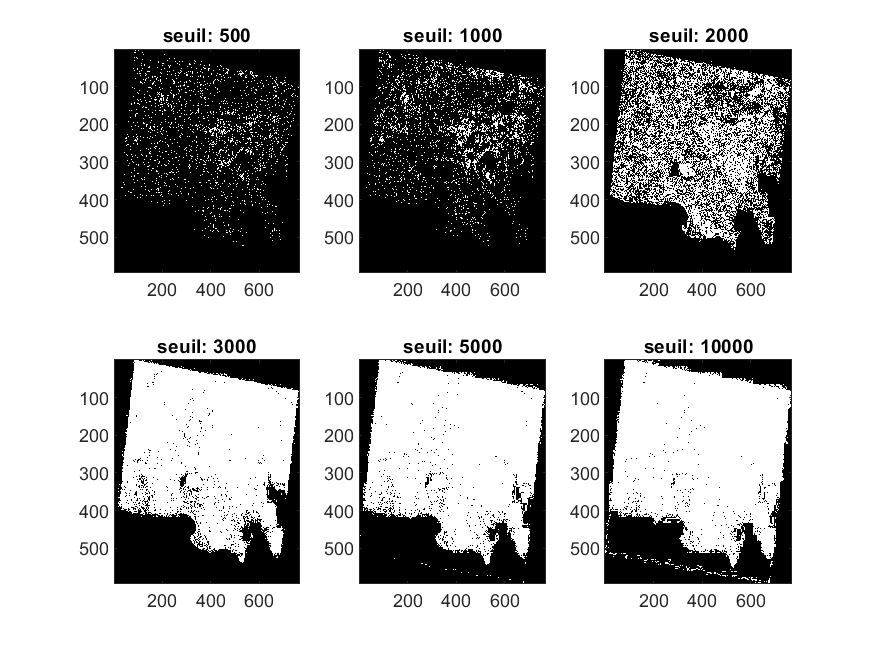
\includegraphics[width=.8\textwidth]{dvi_seuils}
                \centering
            \end{figure}

            On observe alors que :

            \begin{itemize}
                \item{Pour des valeurs trop faibles du seuil on est trop sélectif}
                \item{Pour des valeurs trop élevées du seuil on est trop permissif}
                \item{Pour des valeurs entre ces deux extrêmes on obtient des résultats
                    semblant satisfaisant, par exemple avec ici un seuil valant 2000}
                \item{Les résultats pour des bons choix du seuil semblent meilleurs que ceux
                    obtenus précédemment par seuillage des différents canaux}
            \end{itemize}
        }

    \item{Enfin, on peut envisager une méthode de détection par le biais de la massification
        non-supervisée. On choisit d'utiliser la méthode K-means Clustering.

        Pour une valeur de K donnée, on détermine alors les K classes et on sélectionne
        celle correspondant au DVI le plus important.

        Par exemple, pour $K = 4$, on obtient l'image suivante :

        \begin{figure}[H]
            \caption{Résultat pour $K = 4$}
            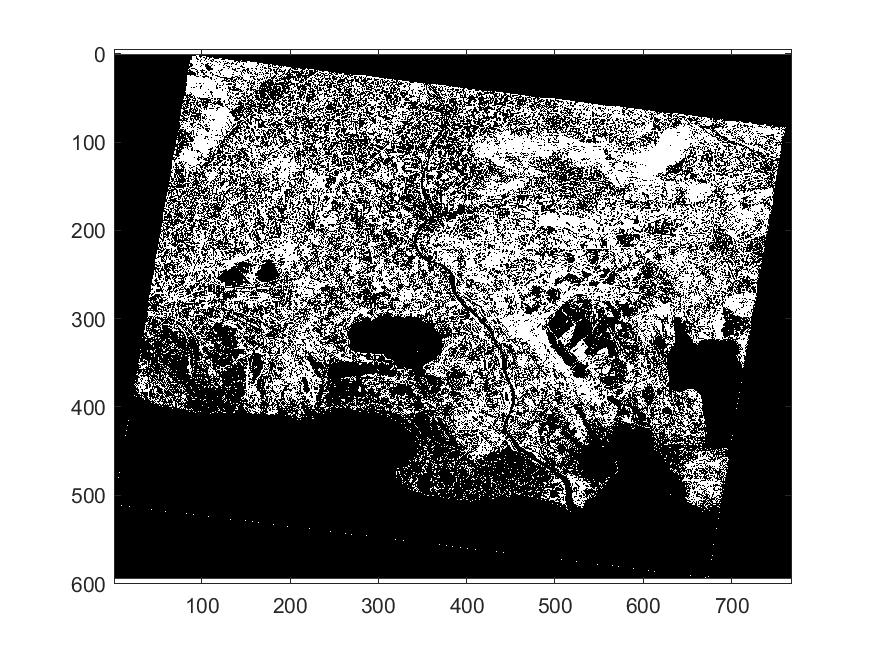
\includegraphics[width=.8\textwidth]{kmeans_1}
            \centering
        \end{figure}

        Pour différentes valeurs de K, on obtient les résultats suivants :

        \begin{figure}[H]
            \caption{Résultats pour différents K}
            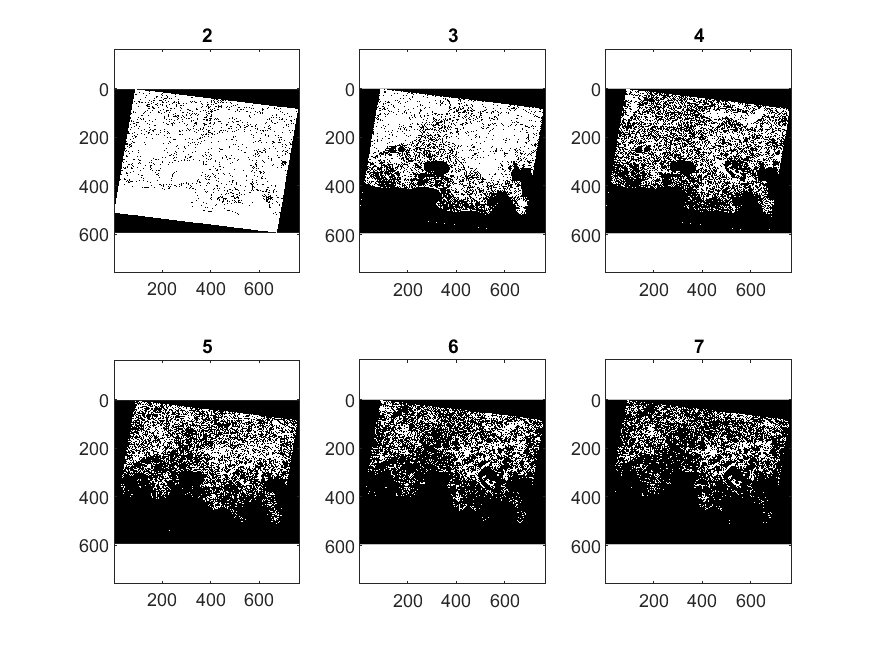
\includegraphics[width=.8\textwidth]{kmeans_2}
            \centering
        \end{figure}

        On observe alors que :

        \begin{itemize}
            \item{Pour des valeurs trop faibles de K, c'est-à-dire pour peu de clusters,
                on obtient pas de bons résultats car le découpage est trop vaste}
            \item{À l'inverse, pour une valeur trop importante de K, on découpe l'image
                en trop de clusters et obtient cette fois trop peu de végétations}
            \item{Pour $K = 3$ ou $K = 4$ dans ce cas on obtient de bons résultats}
        \end{itemize}
        }
\end{enumerate}

\section*{Conclusion}

Pour conclure, lors de ce TP, nous avons pu implémenter différentes méthodes pour la détection
de la végétation : le seuillage d'histogramme, l'utilisation du NDVI et la classification non
supervisée. À partir de l'implémentation de ces méthodes, nous avons en particulier prendre
conscience de l'importance du choix des paramètres vis à vis du résultat qui sera retourné, par
exemple, les valeurs de seuils ou encore, le nombre de clusters. Il convient de toutes les
essayer avec différentes valeurs de paramètres et comparer les résultats pour déterminer
celui qui semble meilleur. En effet, ne disposant pas de vérité terrain, nous ne pouvons
pas déterminer de manière exacte quelle méthode a fourni les meilleurs résultats.

\pagebreak

\begin{appendices}

    \section{Code Matlab}

    \lstinputlisting[language=Matlab]{../main.m}

\end{appendices}

\end{document}
